\chapter{Коптилка}
%\corner{64}
\vepsianrose

Адмирал более\sdash менее выспался, но вылезать из палатки не спешил\mdash снаружи капал дождь. Замполит ещё спал, поэтому, чтобы не будить товарища, он достал судовой журнал и принялся записывать путевые заметки. Он каждый раз брал с собой этот журнал и каждый раз благополучно забывал его вести, но не в этом походе. Он~расписал по~свежим впечатлениям предыдущие два дня и~вспомнил, что обещал команде кофе к завтраку на днёвке.

\diagdash Шурик, там дождь чтоль?\mdash проснулся Замполит.

\diagdash Ну.

\diagdash Неохота вылазить$\ldots$

\diagdash А надо! Я вам кофеёк обещал. И у меня где\sdash то блинная мука была\mdash пойду оладьи соображу, а то каша чемпионов, поди, всем надоела уже.

\diagdash Фигасе разносолы. Я посплю ещё.

\newpage
\begin{wrapfigure}[13]{l}{0.5\textwidth}
	%\begin{figure}[h]
	\centering
	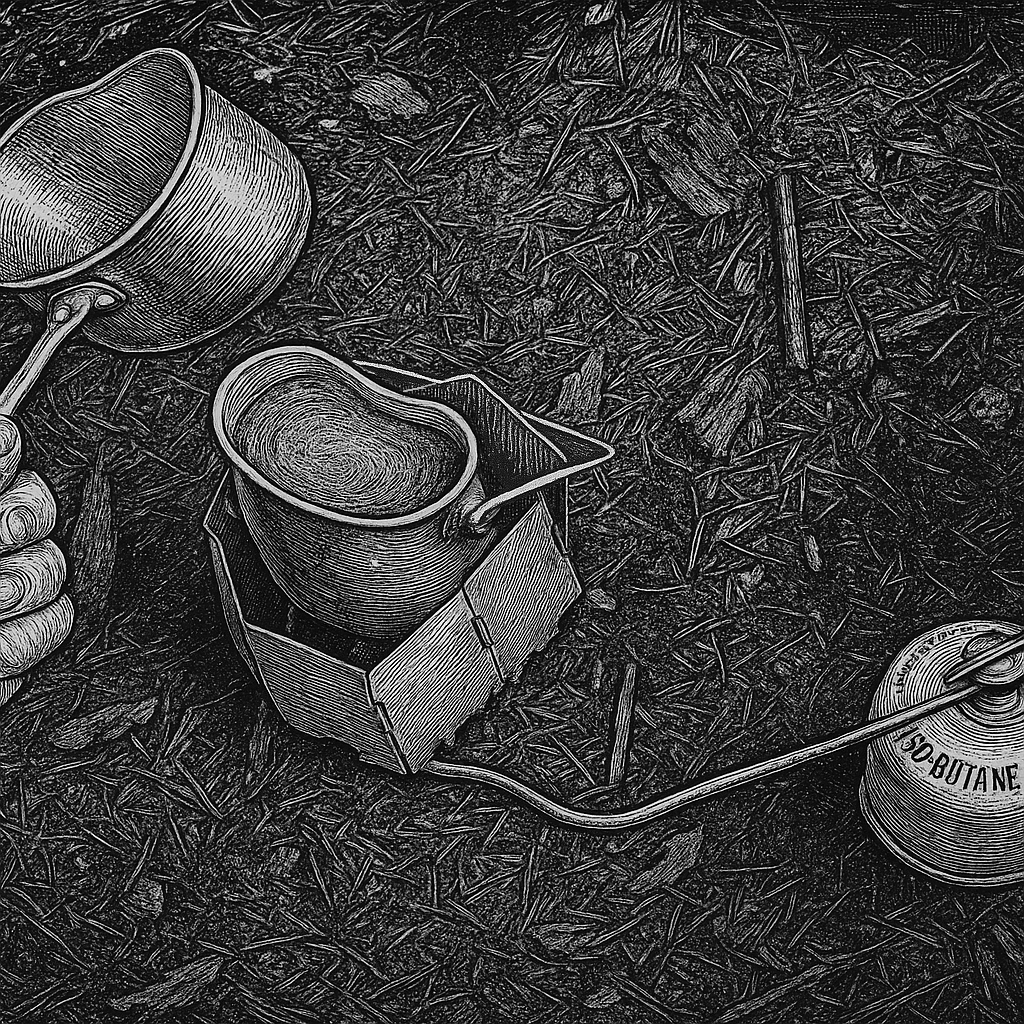
\includegraphics[width=0.47\textwidth]{coffee}
	\caption{\small\textit{...я вам кофеёк обещал...}}
	%\end{figure}
\end{wrapfigure}
Адмирал выполз из~палатки. Дождь почти закончился, но~погодка оставляла желать лучшего\mdash лес вокруг был влажным, дул неслабый ветерочек. Он~распалил костёр из~напиленных вчера впрок дров, поставил воду в~котелке на~чай\mdash всё равно кто\sdash нибудь да захочет чай\mdash и~принялся за кофе. Немного подумав, решил варить кофе на~газу, а~не~на~костре. Для этого он достал и собрал свою мини\sdash горелку, собрал защитный экранчик от ветра, поставил десантный котелок на синий цветок газа, щедро насыпал молотый кофе. Сверху он закрыл котелок подкотельником\mdash получилась как бы крышка\mdash так быстрее закипело. Народ потихонку стал подтягиваться к костру.

\diagdash Шу-у-урик, что варим?\mdash Серёга заспанно приземлился на брёвна.

\diagdash Кофе.

\diagdash Ва-а-ау.

\diagdash Ща, пару сек и будет готово!\mdash Адмирал дождался второго поднятия пенки и стал разливать всем желающим божественный напиток.\mdash Подставляйте!

Кофе вышел шикарным. Адмирал сдобрил его столовой ложкой белорусской сгущёнки и, развалившись в походном кресле, стал наслаждаться моментом.

\newpage

\begin{wrapfigure}[20]{r}{0.58\textwidth}
	%\begin{figure}[h]
	\centering
	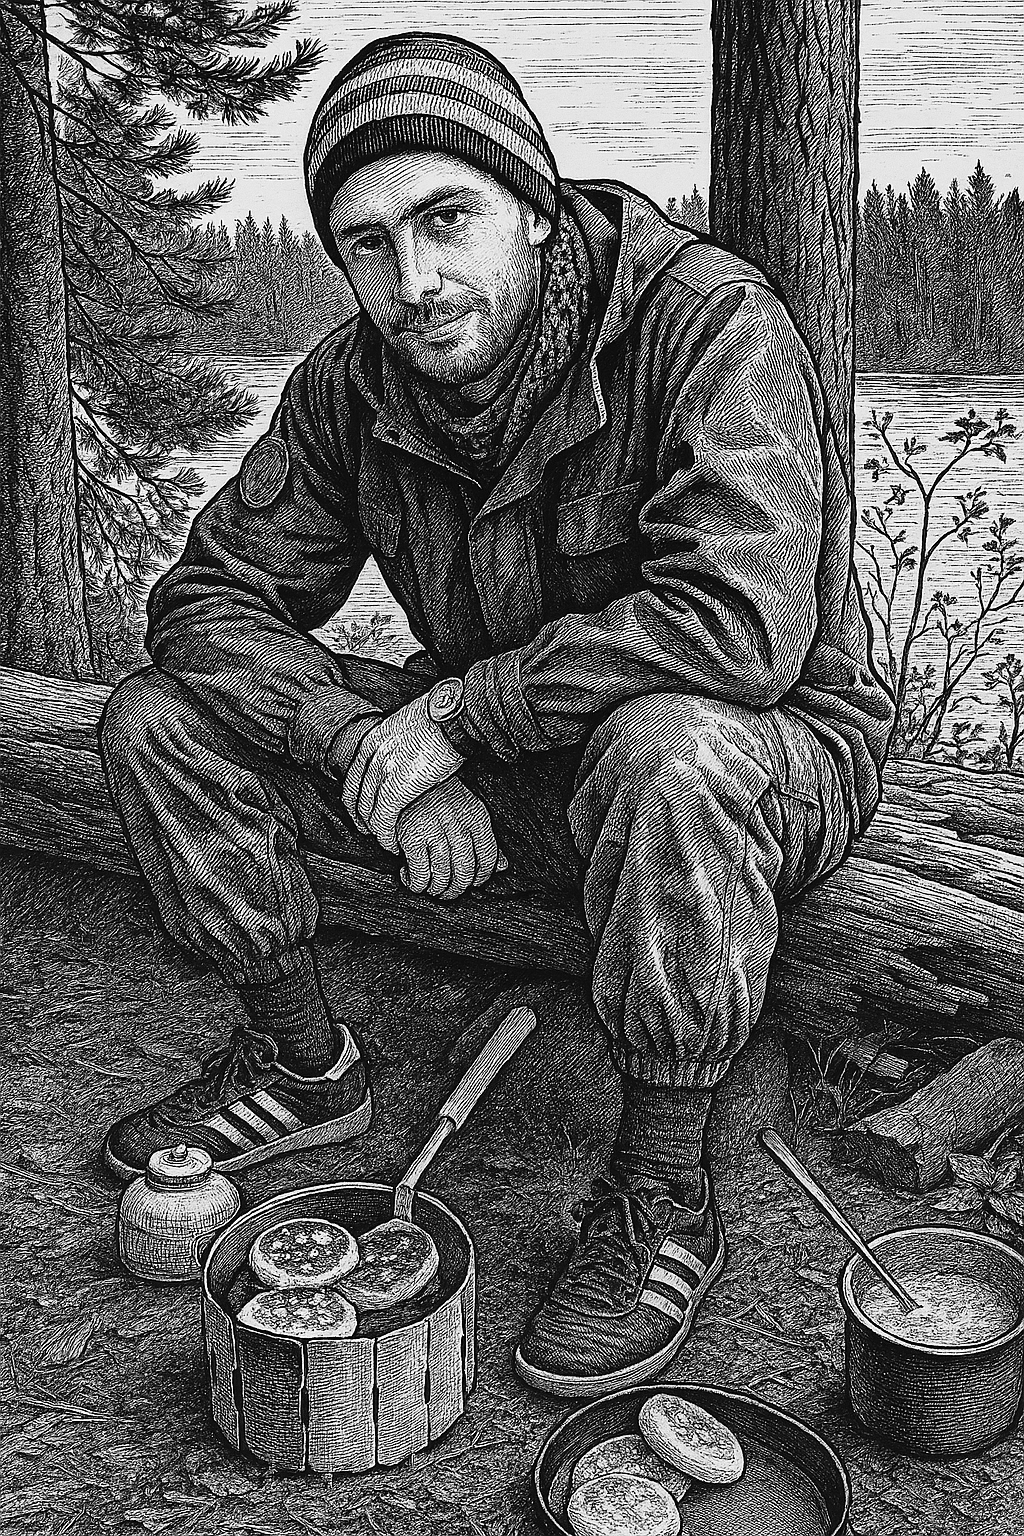
\includegraphics[width=0.56\textwidth]{blinchiki}
	\caption{\small\textit{...принялся за оладьи...}}
	%\end{figure}
\end{wrapfigure}
\diagdash Шурик, такого ты ещё не делал.\mdash изрёк подошедший Замполит, тоже соблазнившись на~кофе.

\diagdash Не, помнишь, мы когда в последний раз по Чагодоще ходили, тоже кофеёк варили как\sdash то?

\diagdash А, тот наш <<арктический>> поход? Смутно~уже.

\diagdash Варили\sdash варили, было дело.\mdash подтвердил Серёга.

\diagdash Ну вот я решил повторить, так сказать.\mdash Адмирал вполне насладился напитком и принялся за оладьи. Он~достал из продуктовой гермы блинную муку и стал читать инструкцию на упаковке.

\diagdash Только не как в прошлый раз, ладно?\mdash посмеиваясь, напомнил Паша эпизод из их сплавного опыта, когда они на~днёвке близ Загривья на Чагодоще неудачно запекли целый котелок с~тестом.

\diagdash Там простая мука была, а то блинная. И сковородка у меня теперь нормальная, не очкуй.\mdash Адмирал согласно инструкции отмерил пропорции и принялся замешивать тесто в~круглом пашином подкотельнике, который как нельзя лучше подошел для этой цели.

Оладьи стали выпекаться вполне себе приличными, Адмирал даже не ожидал. Спустя минут 15 на перевёрнутой крышке котелка образовалась целая горка аппетитно пахнущих оладушек. Паша достал невесть откуда взявшиеся остатки копчёного рулета и прочего по мелочи, народ засел за трапезу.

После все разбрелись кто куда\mdash Замполит с Серёгой взяли пилу и пошли делать <<кружочки>>\mdash спилы сосновых поленьев\mdash на память в качестве сувениров, Руслан в походном кресле кайфовал у костра, Паша отправился на~рыбалку в залив, а Адмирал, сварив себе ещё порцию кофе и~раскурив сигару, снова принялся за путевые заметки.

Серёга с Замполитом напилили <<кружочков>> и~притащили их к костру похвастаться:

\diagdash Мы так, короче, в детстве с каждого сплава притаскивали, потом сушили дома и типа память о~сплаве оставалась.\mdash поделился воспоминаниями с командой Замполит.

\diagdash Сушить только в~пакете надо, наверно, а то треснет спил, наверно.\mdash предположил Серёга.

\diagdash Логично. Надо тоже себе напилить потом.\mdash согласился Адмирал.\mdash Серёг, а ягоды вроде оставались же ещё?\mdash спросил он, повернувшись к тому.

\diagdash Да, вот в пятилитрашке. Компотика наварить?

\diagdash Было бы клёво.

\diagdash Щас сделаем.\mdash Серёга сходил зачерпнул котелок воды.

\begin{wrapfigure}[10]{r}{0.5\textwidth}
	%\begin{figure}[h]
	\centering
	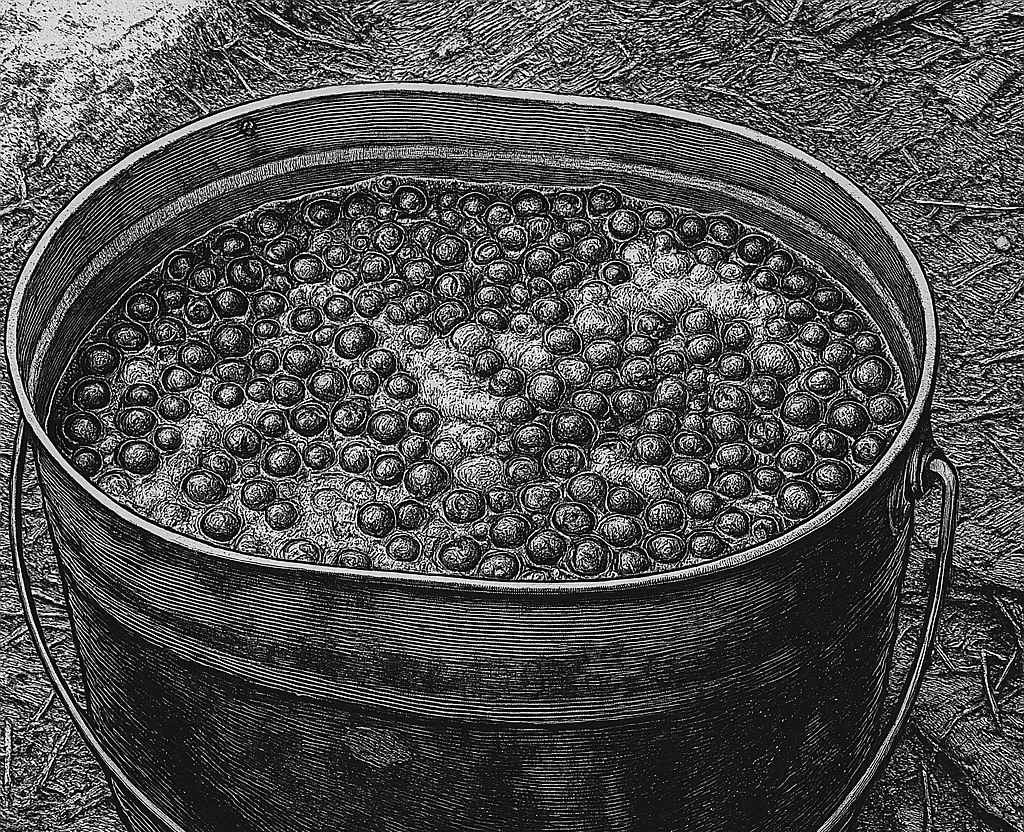
\includegraphics[width=0.48\textwidth]{kompotik}
	\caption{\small\textit{...компотика наварить?...}}
	%\end{figure}
\end{wrapfigure}

Спустя совсем немного времени компот был готов:

\diagdash Нава-а-аристо!

\diagdash А то!

\diagdash Серёга у нас главный по компотам в~этом сплаве.\mdash попробовал компот Руслан.

\diagdash Не, по компотикам главный\mdash Замполит, а Серёга по сборке голубики.\mdash не преминул подколоть Замполита Адмирал.

\diagdash Ой да харош!\mdash Замполит как раз попробовал варево.

\diagdash Ы-ы-ы!

%\diagdash Компот\'{и}н-антипохмел\'{и}н, ы-ы-ы!

\newpage

\begin{wrapfigure}[22]{l}{0.58\textwidth}
	%\begin{figure}[h]
	\centering
	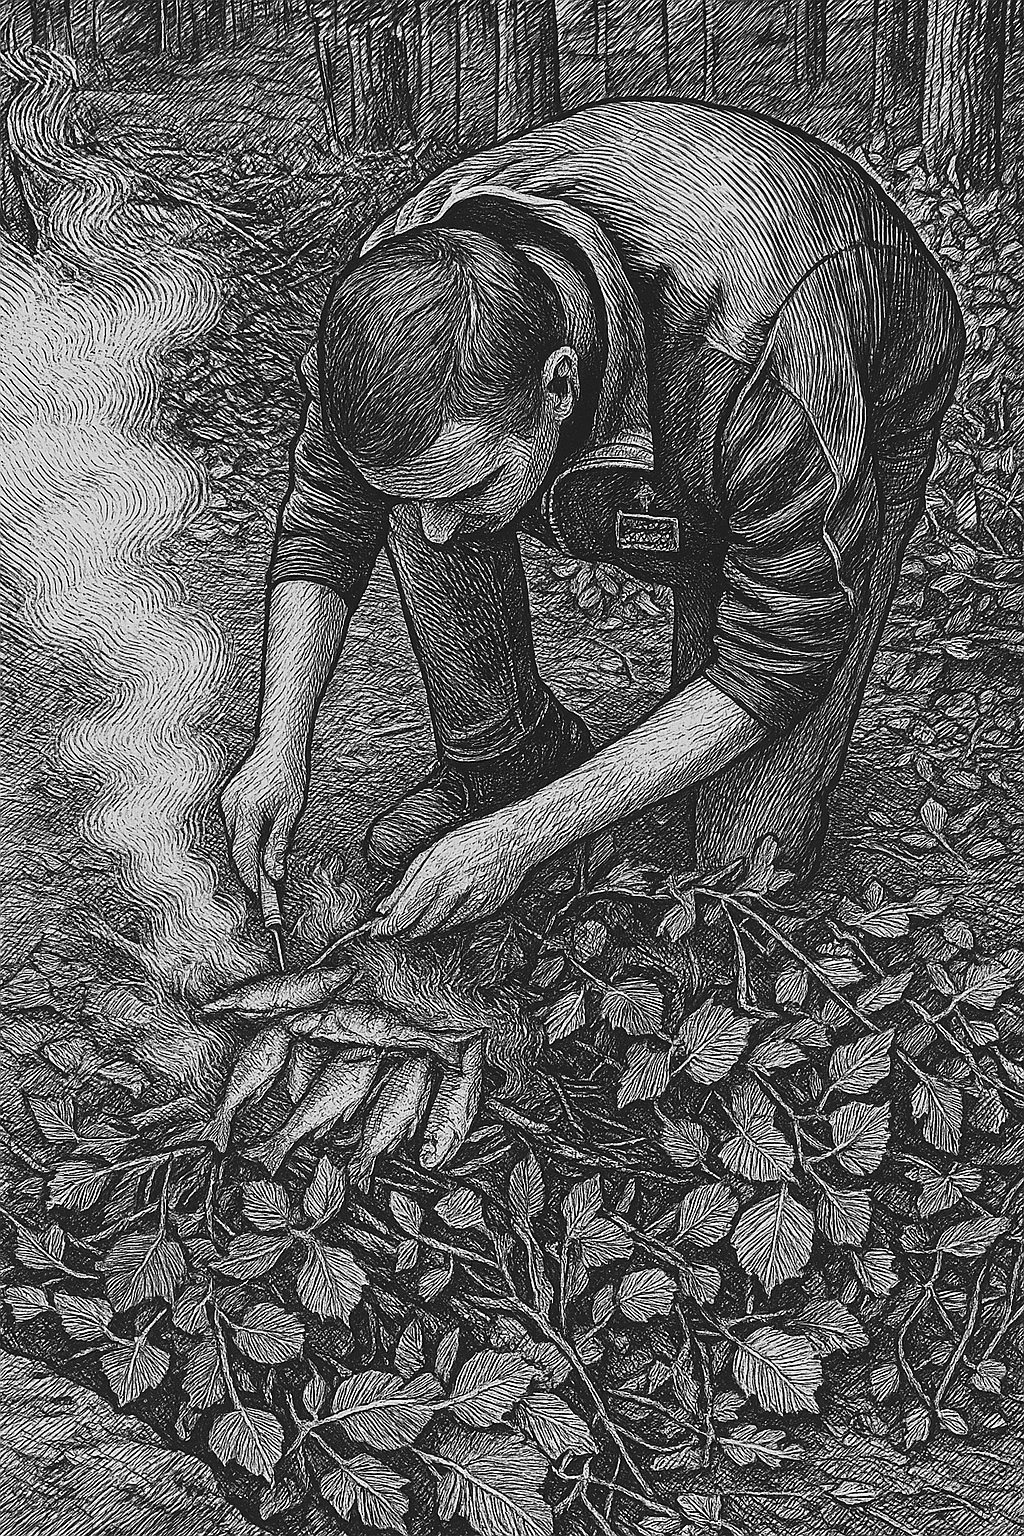
\includegraphics[width=0.56\textwidth]{pashakopt}
	\caption{\small\textit{...Паша стал снимать рыбу...}}
	%\end{figure}
\end{wrapfigure}
ываооывшоа ываы ывщшао ывашгор ываг вргш ывар вышгфр рывы горгшр ш щш щш шщг щшгщшг  гшны ы ываооывшоа ываы ывщшао ывашгор ываг вргш ывар вышгфр рывы горгшр ш щш щш шщг щшгщшг  гшны ы ываооывшоа ываы ывщшао ывашгор ываг вргш ывар вышгфр рывы горгшр ш щш щш шщг щшгщшг  гшны ы ываооывшоа ываы ывщшао ывашгор ываг вргш ывар вышгфр рывы горгшр ш щш щш шщг щшгщшг  гшны ы ываооывшоа ываы ывщшао ывашгор ываг вргш ывар вышгфр рывы горгшр ш щш щш шщг щшгщшг  гшны ы ываооывшоа ываы ывщшао ывашгор ываг вргш ывар вышгфр рывы горгшр ш щш щш шщг щшгщшг  гшны ы ываооывшоа ываы ывщшао ывашгор ываг вргш ывар вышгфр рывы горгшр 

ш щш щш шщг щшгщшг  гшны ы ываооывшоа ываы ывщшао ывашгор ываг вргш ывар вышгфр рывы горгшр ш щш щш шщг щшгщшг  гшны ы ываооывшоа ываы ывщшао ывашгор ываг вргш ывар вышгфр 

\newpage

\begin{wrapfigure}[11]{l}{0.58\textwidth}
	%\begin{figure}[h]
	\centering
	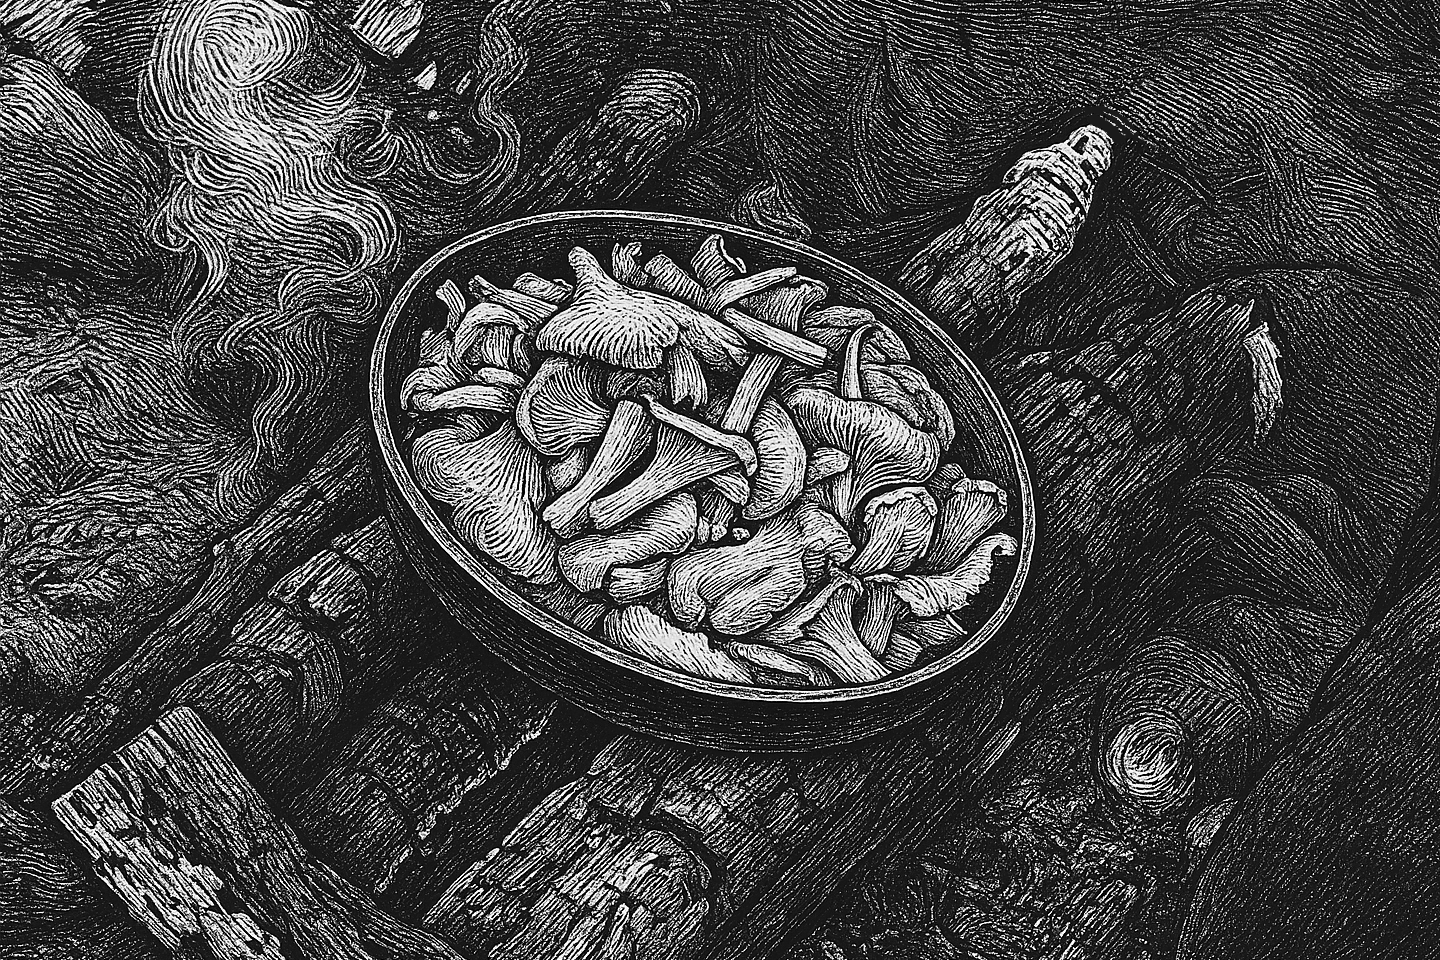
\includegraphics[width=0.56\textwidth]{lisich}
	\caption{\small\textit{...зажарили лисички...}}
	%\end{figure}
\end{wrapfigure}
ывар вышгфр рывы горгшр ш щш щш шщг щшгщшг  гшны ы ываооывшоа ываы ывщшао ывашгор ываг вргш ывар вышгфр рывы горгшр ш щш щш шщг щшгщшг  гшны ы ываооывшоа ываы ывщшао ывашгор ываг вргш ывар вышгфр рывы горгшр ш щш щш шщг щшгщшг  гшны ы ываооывшоа ываы ывщшао 

ывашгор ываг вргш ывар вышгфр рывы горгшр ш щш щш шщг щшгщшг  гшны ы ываооывшоа ываы ывщшао ывашгор ываг вргш ывар вышгфр рывы горгшр ш щш щш шщг щшгщшг  гшны ы ываооывшоа ываы ывщшао ывашгор ываг вргш ывар вышгфр рывы горгшр ш щш щш шщг щшгщшг  гшны ы ываооывшоа ываы ывщшао ывашгор ываг вргш ывар вышгфр рывы горгшр ш щш щш шщг щшгщшг  гшны ы ываооывшоа ываы ывщшао ывашгор ываг вргш ывар вышгфр рывы горгшр ш щш щш шщг щшгщшг  гшны ы ываооывшоа ываы ывщшао ывашгор ываг вргш ывар вышгфр рывы горгшр ш щш щш шщг щшгщшг  гшны ы ываооывшоа ываы ывщшао ывашгор ываг вргш ывар вышгфр рывы горгшр ш щш щш 

\newpage

\begin{wrapfigure}[12]{l}{0.58\textwidth}
	%\begin{figure}[h]
	\centering
	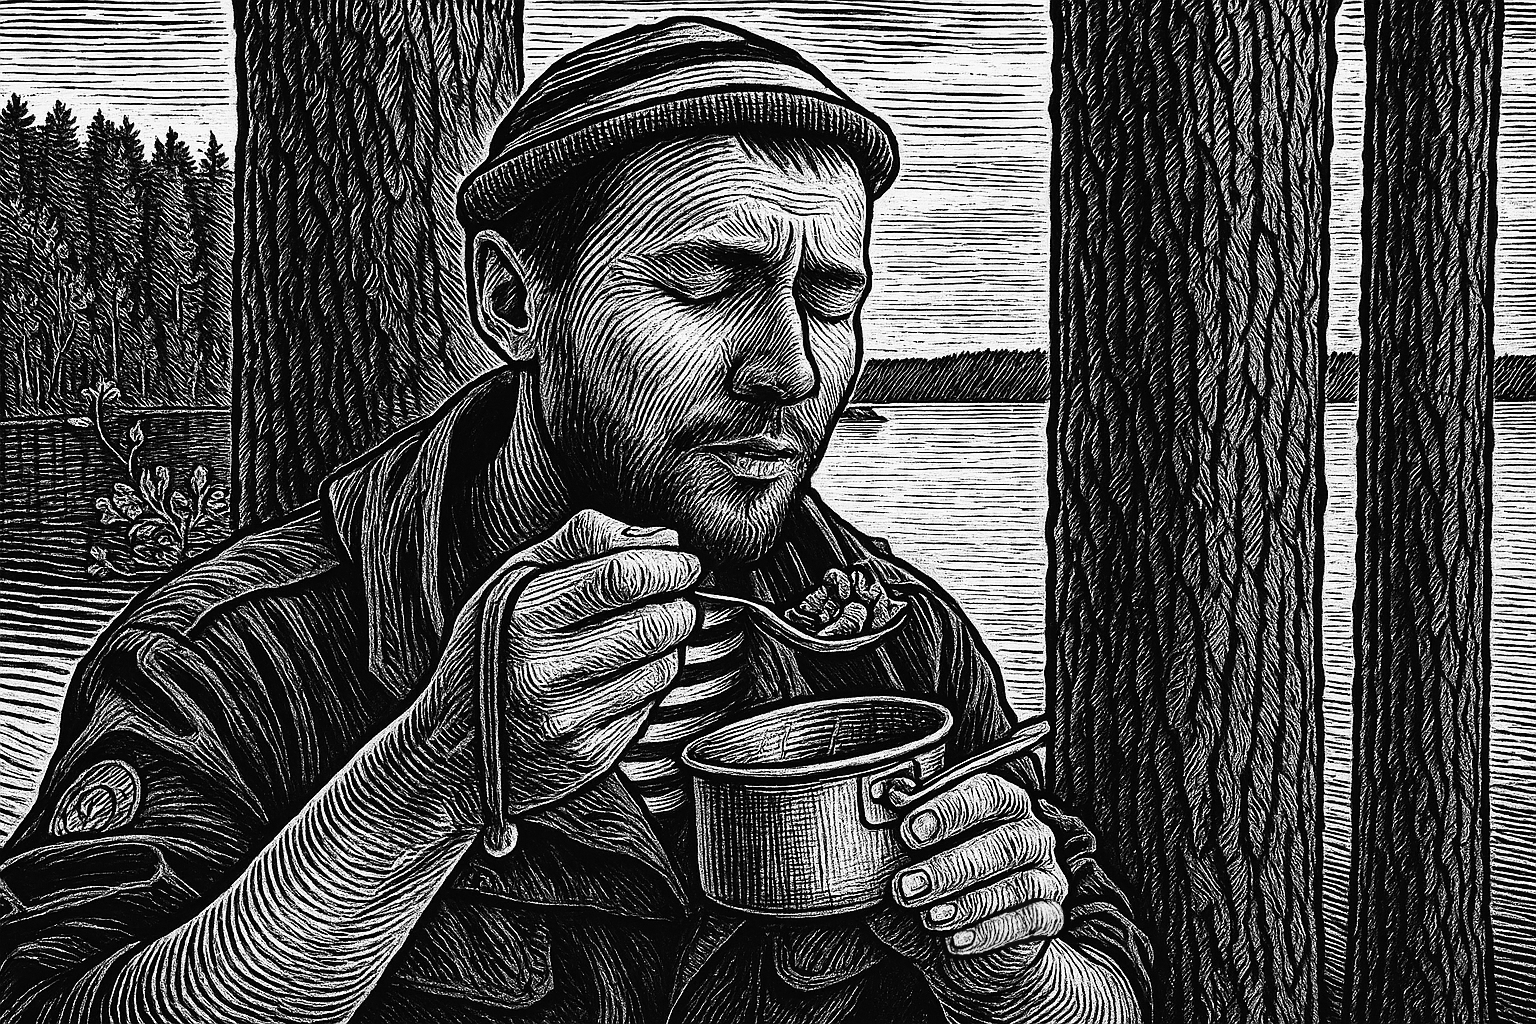
\includegraphics[width=0.56\textwidth]{lisichnum}
	\caption{\small\textit{...Адмирал закрыл глаза...}}
	%\end{figure}
\end{wrapfigure}
шщг щшгщшг  гшны ы ываооывшоа ываы ывщшао ывашгор ываг вргш ывар вышгфр рывы горгшр ш щш щш шщг щшгщшг  гшны ы ываооывшоа ываы ывщшао ывашгор ываг вргш ывар вышгфр рывы горгшр ш щш щш шщг щшгщшг  гшны ы ываооывшоа ываы ывщшао ывашгор ываг вргш ывар вышгфр рывы горгшр ш щш щш шщг щшгщшг  гшны ы ываооывшоа ываы ывщшао ывашгор ываг вргш ывар вышгфр рывы горгшр ш щш щш шщг щшгщшг  гшны ы ываооывшоа ываы ывщшао ывашгор ываг вргш ывар вышгфр рывы горгшр ш щш щш шщг щшгщшг  гшны ы ываооывшоа ываы ывщшао ывашгор ываг вргш ывар вышгфр рывы горгшр ш щш щш шщг щшгщшг  гшны ы ываооывшоа ываы ывщшао ывашгор ываг вргш ывар вышгфр рывы горгшр ш щш щш шщг щшгщшг  гшны ы ываооывшоа ываы ывщшао ывашгор ываг вргш ывар вышгфр рывы горгшр ш щш щш шщг щшгщшг  гшны ы ываооывшоа ываы ывщшао ывашгор ываг вргш ывар вышгфр рывы горгшр ш щш щш шщг щшгщшг  гшны ы 




\begin{center}
	\psvectorian[scale=0.4]{88} % Красивый вензелёк :)
\end{center}
